Eq \eqref{eq:solutions/3/4/8/eq:a0} cab be written as
\begin{align}
\vec{x}^T\vec{x}+\myvec{\frac{7}{2}&\frac{5}{2}}\vec{x}-\frac{13}{2}=0\\
\implies \vec{x}^T\vec{x}+2\myvec{\frac{7}{4}&\frac{5}{4}}\vec{x}-\frac{13}{2}=0
\label{eq:solutions/3/4/8/eq:a2}
\end{align}
The above eq \eqref{eq:solutions/3/4/8/eq:a2} cab be compared with the circle equation gives as
\begin{align}
\vec{x}^T\vec{x}+2\vec{u}^T\vec{x}+f=0
\label{eq:solutions/3/4/8/eq:a3}
\end{align}
\begin{figure}[!ht]
	\centering
	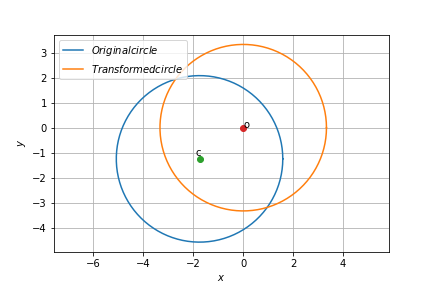
\includegraphics[width=\columnwidth]{./solutions/3/4/8/circle.png}
	\caption{Figure depicting transformation of circle}
	\label{eq:solutions/3/4/8/myfig}
\end{figure}
then
\begin{align}
\vec{u} = \myvec{\frac{7}{4}\\\frac{5}{4}}\\
\label{eq:solutions/3/4/8/eq:a4}
\implies centre, \vec{c} = \myvec{\frac{-7}{4}\\\frac{-5}{4}}\\
\norm{u}^2 - r^2 = f\\
\implies r^2 = \norm{u}^2 - f\\
\implies r^2 = \left(\frac{7}{4}\right)^2+\left(\frac{5}{4}\right)^2+\frac{13}{2}\\
\implies radius, r = \sqrt{\frac{89}{8}}
\end{align}
The eq \eqref{eq:solutions/3/4/8/eq:a1} can be written by changing the origin as
\begin{align}
\vec{(x+c)}^T\vec{(x+c)} = \frac{89}{8}\\
\implies \vec{x}^T\vec{x}+\vec{x}^T\vec{c}+\vec{c}^T\vec{x}+\vec{c}^T\vec{c} = \frac{89}{8}
\label{eq:solutions/3/4/8/eq:a5}
\end{align}
We know that
\begin{align}
\vec{x}^T\vec{c} = \vec{c}^T\vec{x}
\label{eq:solutions/3/4/8/eq:a6}
\end{align}
by substituting \eqref{eq:solutions/3/4/8/eq:a6} in \eqref{eq:solutions/3/4/8/eq:a5}
\begin{align}
\vec{x}^T\vec{x}+2\vec{c}^T\vec{x}+\vec{c}^T\vec{c} = \frac{89}{8}
\label{eq:solutions/3/4/8/eq:a7}
\end{align}
substituting the orgin of \eqref{eq:solutions/3/4/8/eq:a0} in above eq \eqref{eq:solutions/3/4/8/eq:a7}
\begin{align}
\vec{x}^T\vec{x}+2\myvec{\frac{7}{4}&\frac{5}{4}}\vec{x}+\myvec{\frac{-7}{4}&\frac{-5}{4}}\myvec{\frac{-7}{4}\\\frac{-5}{4}} = \frac{89}{8}\\
\implies \vec{x}^T\vec{x}+\myvec{\frac{7}{2}&\frac{5}{2}}\vec{x}+\frac{74}{16}-\frac{89}{8} = 0\\
\implies \vec{x}^T\vec{x}+\myvec{\frac{7}{2}&\frac{5}{2}}\vec{x}-\frac{13}{2} = 0\\
\implies 2\vec{x}^T\vec{x}+\myvec{7&5}\vec{x}-13 = 0
\end{align}
$\therefore$ It is proved that by changing the origin in \eqref{eq:solutions/3/4/8/eq:a1} we obtained \eqref{eq:solutions/3/4/8/eq:a0}.
